\cleardoublepage

\chapter{Results and Analysis}
\label{chapter:results}
This section contains a complete description of the test problems for modeling as well as results from numerical studies.
To illustrate the performance of using the DMD-PM(n) method and the DMD-FPM(n) method, several test problems were analyzed. 
In all cases, the fundamental eigenmode was computed using a power method implementation as the benchmark and the snapshot generator for use with DMD. 

\section{Test problem}
The test problems considered are (1) the 2-D, IAEA diffusion benchmark\cite{center1977benchmark}, (2) a 1-D, 70-pin BWR core model\citep{rahnema_generalized_2008}, and (3) the 2-D C5G7 benchmark\cite{oecd_nuclear_energy_agency_benchmark_2003}.
Problem(1) is used to test the DMD-PM(n) method, and Problem(2) Problem(3) are used to test the DMD-FPM(n) method.
\subsection{Test problem for DMD-PM(n)}
The well-known, two-dimensional (2-D) International Atomic Energy Agency (IAEA) diffusion benchmark was used to test the DMD acceleration algorithm proposed in \CHAPTER{chapter:DMD-PM}.
The governing diffusion equations are
\begin{equation}
 \begin{split}
  -\nabla D(\mathbf{r})_1 \nabla \phi_1 (\mathbf{r}) + \Sigma_{r1}(\mathbf{r}) \phi_1 (\mathbf{r}) 
    &= \frac{1}{k} \left (\nu\Sigma_{f1}\phi_1(\mathbf{r}) + \nu\Sigma_{f2}\phi_2(\mathbf{r}) \right ) \\
 -\nabla D(\mathbf{r})_2 \nabla \phi_2 (\mathbf{r}) + \Sigma_{a2}(\mathbf{r}) \phi_2 (\mathbf{r}) 
    &= \Sigma_{s1\to 2}\phi_1(\mathbf{r}) \, ,
 \end{split}
 \label{eq:twogroupdiff}
\end{equation}
where the notation defined in \CHAPTER{chapter:multigroup}.
All parameters including the cross sections are defined in the technical report published from Argonne National Laboratory.
The basic core layout is shown in \FIGURE{fig:IAEA}, where the west and south boundary are reflective, and the north and east boundary are vacuum.

\begin{figure*}[htb!]
\centering
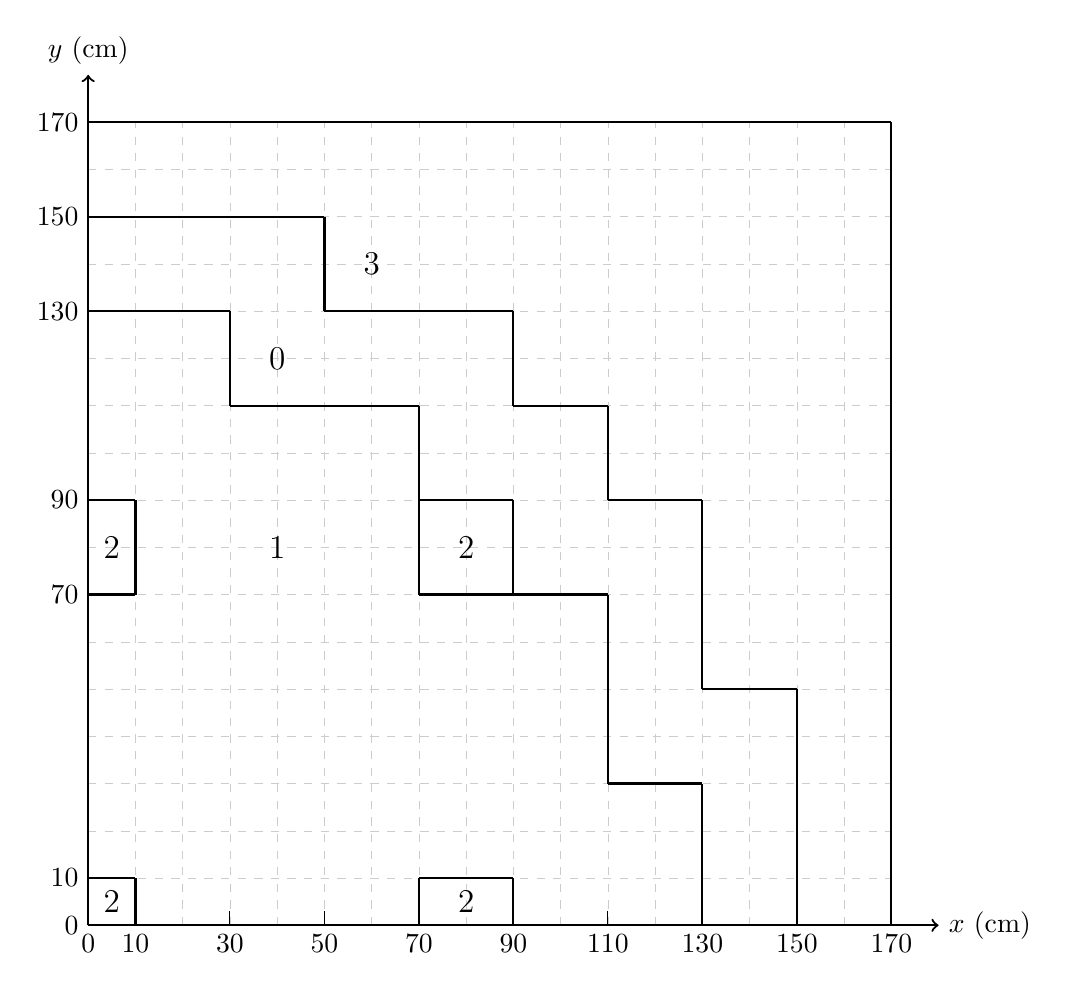
\begin{tikzpicture}[scale=.6]
\begin{scope}<->;
% GRID
 \draw[step=1.0,gray,very thin, dashed,opacity=0.4] (0.0,0.0) grid (17.0, 17.0); 
  
% AXES
  \draw[black, thick, ->] (0, 0) -- (18,  0) node[right] {$x$ (cm)};
  \draw[black, thick, ->] (0, 0) -- ( 0, 18) node[above] {$y$ (cm)};

% Material 3 regions
  \draw[black, thick] (  0.0, 17.0) -- (17.0, 17.0);
  \draw[black, thick] (  17.0, 17.0) -- (17.0, 0.0);  
  \node[font=\large] at (6.0, 14.0) {3};

% Material 0 regions
  \draw[black, thick] (  0.0, 15.0) -- (5.0, 15.0);
  \draw[black, thick] (  5.0, 15.0) -- (5.0, 13.0);  
  \draw[black, thick] (  5.0, 13.0) -- (9.0, 13.0);
  \draw[black, thick] (  9.0, 13.0) -- (9.0, 11.0);
  \draw[black, thick] (  9.0, 11.0) -- (11.0, 11.0); 
  \draw[black, thick] (  11.0, 11.0) -- (11.0, 9.0); 
  \draw[black, thick] (  11.0, 9.0) -- (13.0, 9.0); 
  \draw[black, thick] (  13.0, 9.0) -- (13.0, 5.0);
  \draw[black, thick] (  15.0, 5.0) -- (13.0, 5.0);
  \draw[black, thick] (  15.0, 5.0) -- (15.0, 0.0);
  \node[font=\large] at (4.0, 12.0) {0};

% Material 1 regions
  \draw[black, thick] (  0.0, 13.0) -- (3.0, 13.0);
  \draw[black, thick] (  3.0, 13.0) -- (3.0, 11.0);  
  \draw[black, thick] (  3.0, 11.0) -- (7.0, 11.0);
  \draw[black, thick] (  7.0, 11.0) -- (7.0, 7.0);
  \draw[black, thick] (  7.0, 7.0) -- (11.0, 7.0); 
  \draw[black, thick] (  11.0, 7.0) -- (11.0, 3.0);  
  \draw[black, thick] (  11.0, 3.0) -- (13.0, 3.0);  
  \draw[black, thick] (  13.0, 3.0) -- (13.0, 0.0);  
  \node[font=\large] at (4.0, 8.0) {1};

% Material 2 regions
  \draw[black, thick] (  0.0, 0.0) -- (0.0, 1.0);
  \draw[black, thick] (  1.0, 1.0) -- (1.0, 0.0);  
  \draw[black, thick] (  0.0, 1.0) -- (1.0, 1.0);
  \node[font=\large] at (0.5, 0.5) {2};  
  
  \draw[black, thick] (  0.0, 7.0) -- (1.0, 7.0); 
  \draw[black, thick] (  1.0, 7.0) -- (1.0, 9.0);  
  \draw[black, thick] (  1.0, 9.0) -- (0.0, 9.0);  
  \node[font=\large] at (0.5, 8.0) {2};  
  
  
  \draw[black, thick] (  7.0, 7.0) -- (9.0, 7.0);  
  \draw[black, thick] (  9.0, 7.0) -- (9.0, 9.0);  
  \draw[black, thick] (  9.0, 9.0) -- (7.0, 9.0);  
  \node[font=\large] at (8.0, 8.0) {2};

  \draw[black, thick] (  7.0, 0.0) -- (9.0, 0.0);
  \draw[black, thick] (  9.0, 0.0) -- (9.0, 1.0);
  \draw[black, thick] (  9.0, 1.0) -- (7.0, 1.0);
  \draw[black, thick] (  7.0, 1.0) -- (7.0, 0.0);
  \node[font=\large] at (8.0, 0.5) {2}; 
 
% ticks
  \foreach \x/\xtext in {0, 10, 30, 50, 70, 90, 110, 130, 150, 170}
      \draw[black,xshift=0.1*\x cm] (0,.3) -- (0,0) node[below] {$\xtext$};
  \foreach \y/\ytext in {0, 10, 70, 90, 130, 150, 170}
      \draw[black,yshift=0.1*\y cm] (.3,0) -- (0,0) node[left] {$\ytext$};

\end{scope}
\end{tikzpicture}
\caption{Geometry as modeled for the IAEA 2-D diffusion benchmark.  Material properties can be found in the benchmark documentation.  Materials 0 and 1 are fuel, material 2 represents control, while material 3 represents the outer reflector.}
\label{fig:IAEA}
\end{figure*}

The mesh-center, finite-volume approximation was employed on a uniform, 45 $\times$ 45 spatial mesh.
The discrete ordinates transport code DETRAN was used to generate the explicit system matrix $\mathbf{A}$.
Upon discretization, the entire set of equations was cast in terms of the fission source density, i.e., $\mathbf{f} = \nu\Sigma_{f1}\phi_1(\mathbf{r}) + \nu\Sigma_{f2}\phi_2(\mathbf{r})$, which results in a $2025 \times 2025$ operator. 
Hence, problem(1) is not large, but it proved to be a valuable test case for the method, and, therefore, ensured a reasonable computing time while debugging the code.

%Note that the eigenvalue is typically updated by fission rate.
%At the time of the study, the in-house transport solver used the ratio of fluxes for the eigenvalue update.
%However, the code has since been updated to use the ratio of fission densities, and found a negligible difference in results.

All calculations were initialized with a vector in which each element was sampled from the uniform distribution $U[0, 1]$. 
This randomized starting vector helps to ensure that all eigenmodes can be present.
A formal sensitivity study was not performed to understand how this initial guess impacts the algorithm performance, but scoping studies suggest there is little impact on the number of iterations required for any particular algorithm.
In this case, a reference solution was computed using the implicitly-restarted Arnoldi method as implemented in SciPy \cite{scipy}.
All DMD calculations were performed using the Python package {\tt PyDMD} \cite{pydmd}.

\subsection{Test problem for DMD-FPM(n)}

To illustrate the performance of this method, a simple 1-D test problem was designed to resemble a slab BWR core.
This testing case was adapted from previous, transport applications from \citet{rahnema_generalized_2008}. 
The geometry of the 2-group BWR test case is shown in \FIG{fig:BWRconfig}.
\begin{figure*}[htb!]
    \centering
    \begin{minipage}[c]{\textwidth}
        \centering
        \includestandalone[mode=buildnew, width=0.85\linewidth]{tex/figures/core1}
    \end{minipage}
    \begin{minipage}[c]{\textwidth}
        \centering
        \includestandalone[mode=buildnew, width=0.3\linewidth]{tex/figures/assemblies}
    \end{minipage}
    \begin{minipage}[c]{\textwidth}
        \centering
        \includestandalone[mode=buildnew, width=0.7\linewidth]{tex/figures/core_materials}
    \end{minipage}
    \caption{Configuration for the BWR Test Problem}
    \label{fig:BWRconfig}
\end{figure*}

This core configuration had two unique assemblies.  
Three fuel types were used, including  4.5 \% enriched $UO_2$ , 2.5\% enriched $UO_2$ , and 4.5 \% enriched $UO_2$ with 5 wt\% $Gd_2O_3$.
Fuel pins for this problem were 3.2512 cm thick with 1.1176 cm of moderator on each side.
The baseline pincell discretization consisted of 18 mesh cells of fuel enclosed by six mesh cells of moderator;therefore, each pincell contained 30 mesh points.
Boundary conditions on both sides for this case were vacuum.

The final test problem was the well-studied 2-D C5G7 benchmark \cite{oecd_nuclear_energy_agency_benchmark_2003}, which was used to verify the performance of algorithm for multi-dimensional problems.
The configuration of the benchmark was adapted from \citet{reed_2015}.
The configuration of a quarter core contains four fuel-pin assemblies and five moderator assemblies as shown in \FIGURE{fig:C5G7_config}.
Each fuel assembly used 17 $\times$ 17 individual pincells, and the geometry of a $UO_2$ assembly is shown in \FIG{fig:UO2_config}, while that of a MOX assembly is shown in \FIG{fig:MOX_config}.
Here, each pincell is discretized on a 7$\times$7 Cartesian mesh.
The dimensions are shown in \FIG{fig:MOX_config}.
\begin{figure*}[htb]
    \centering
    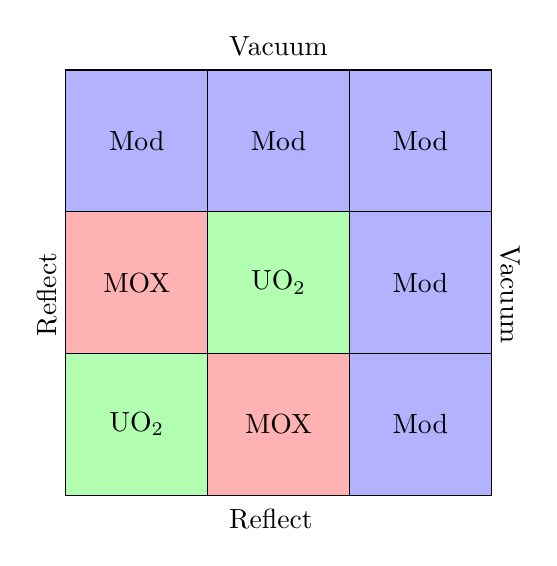
\begin{tikzpicture}[scale=0.6, every node/.style={scale=1}]
        \filldraw[xshift=6 cm, yshift=0 cm, fill=blue!30!white, draw=black] 
        (0, 0) rectangle (3,3) node[pos=.5] {Mod};
        \filldraw[xshift=6 cm, yshift=3 cm, fill=blue!30!white, draw=black] 
        (0, 0) rectangle (3,3) node[pos=.5] {Mod};
        \filldraw[xshift=6 cm, yshift=6 cm, fill=blue!30!white, draw=black] 
        (0, 0) rectangle (3,3) node[pos=.5] {Mod};
        \filldraw[xshift=3 cm, yshift=6 cm, fill=blue!30!white, draw=black] 
        (0, 0) rectangle (3,3) node[pos=.5] {Mod};
        \filldraw[xshift=0 cm, yshift=6 cm, fill=blue!30!white, draw=black] 
        (0, 0) rectangle (3,3) node[pos=.5] {Mod};
        \filldraw[xshift=0 cm, yshift=0 cm, fill=green!30!white, draw=black] 
        (0, 0) rectangle (3,3) node[pos=.5] {UO$_2$};
        \filldraw[xshift=3 cm, yshift=3 cm, fill=green!30!white, draw=black] 
        (0, 0) rectangle (3,3) node[pos=.5] {UO$_2$};
        \filldraw[xshift=3 cm, yshift=0 cm, fill=red!30!white, draw=black] 
        (0, 0) rectangle (3,3) node[pos=.5] {MOX};
        \filldraw[xshift=0 cm, yshift=3 cm, fill=red!30!white, draw=black] 
        (0, 0) rectangle (3,3) node[pos=.5] {MOX};
        \draw[xshift=9cm,yshift=4.25cm] node[right] 
        {\rotatebox{-90}{Vacuum}};
        \draw[yshift=4.25cm] node[left] {\rotatebox{90}{Reflect}};
        \draw[xshift=3.25cm,yshift=9.5cm] node[right] {{Vacuum}};
        \draw[xshift=3.25cm, yshift=-.5cm] node[right] {{Reflect}};
    \end{tikzpicture}
    \caption{Configuration for the C5G7 benchmark.  Each square represents the area of a 
             $17\times17$ pin assembly}
    \label{fig:C5G7_config}
\end{figure*}

\begin{figure*}[htb]
    \centering
    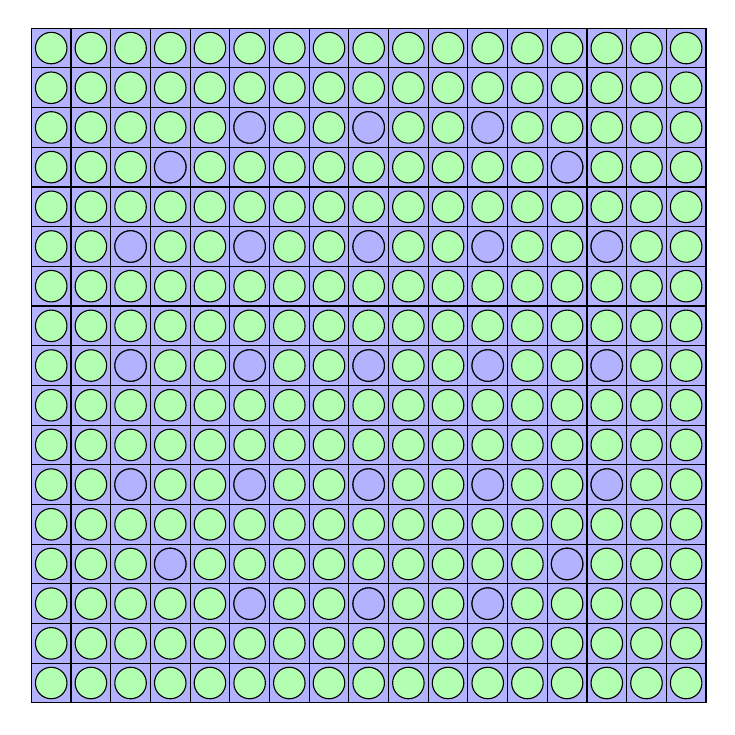
\begin{tikzpicture}[scale=0.4, every node/.style={scale=1}]
        \foreach \x in {0,1.26,...,20.16}
        \foreach \y in {0,1.26,...,20.16}
        \filldraw[xshift=\x cm, yshift=\y cm, fill=blue!30!white, 
        draw=black] (0, 0) rectangle (1.26,1.26) node[pos=.5] {};
        \foreach \x in {0,1.26,...,20.16}
        \foreach \y in {0,1.26,...,20.16}
        \filldraw[xshift=\x cm, yshift=\y cm, fill=green!30!white, 
        draw=black] (.63,.63) circle (.5) node[pos=.5] {};
        \foreach \x in {5*1.26, 8*1.26, 11*1.26}
        \foreach \y in {2*1.26, 14*1.26}
        \filldraw[xshift=\x cm, yshift=\y cm, fill=blue!30!white, 
        draw=black] (.63,.63) circle (.5) node[pos=.5] {};
        \foreach \x in {3*1.26, 13*1.26}
        \foreach \y in {3*1.26, 13*1.26}
        \filldraw[xshift=\x cm, yshift=\y cm, fill=blue!30!white, 
        draw=black] (.63,.63) circle (.5) node[pos=.5] {};
        \foreach \x in {2*1.26, 5*1.26, 8*1.26, 11*1.26, 14*1.26}
        \foreach \y in {5*1.26, 8*1.26, 11*1.26}
        \filldraw[xshift=\x cm, yshift=\y cm, fill=blue!30!white, 
        draw=black] (.63,.63) circle (.5) node[pos=.5] {};
    \end{tikzpicture}
    \caption{Configuration for a UO$_2$ fuel bundle.  The green represents a 
             UO$_2$ pincell, while the blue represents a guide tube modeled as 
             a pincell filled with moderator}
    \label{fig:UO2_config}
\end{figure*}

\begin{figure*}[htb]
    \centering
    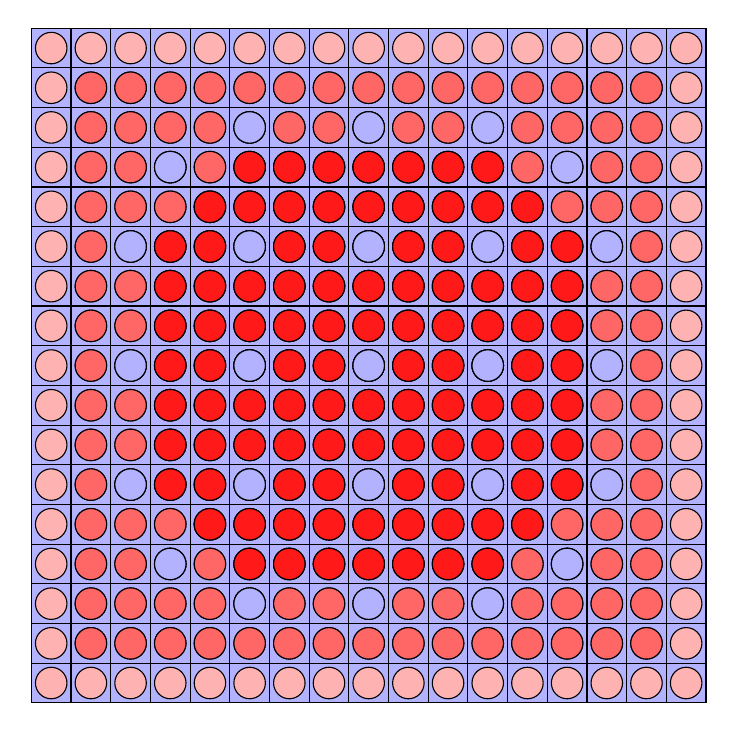
\begin{tikzpicture}[scale=0.4, every node/.style={scale=1}]
        \foreach \x in {0,1.26,...,20.16}
        \foreach \y in {0,1.26,...,20.16}
        \filldraw[xshift=\x cm, yshift=\y cm, fill=blue!30!white, 
        draw=black] (0, 0) rectangle (1.26,1.26) node[pos=.5] {};
        \foreach \x in {0,1.26,...,20.16}
        \foreach \y in {0,1.26,...,20.16}
        \filldraw[xshift=\x cm, yshift=\y cm, fill=red!30!white, draw=black] 
        (.63,.63) circle (.5) node[pos=.5] {};
        \foreach \x in {1.26,2.52,...,20.16}
        \foreach \y in {1.26,2.52,...,20.16}
        \filldraw[xshift=\x cm, yshift=\y cm, fill=red!60!white, draw=black] 
        (.63,.63) circle (.5) node[pos=.5] {};
        \foreach \x in {5*1.26,6*1.26,7*1.26,8*1.26,9*1.26,10*1.26,11*1.26}
        \foreach \y in {3*1.26,13*1.26}
        \filldraw[xshift=\x cm, yshift=\y cm, fill=red!90!white, draw=black] 
        (.63,.63) circle (.5) node[pos=.5] {};
        \foreach \x in 
        {4*1.26,5*1.26,6*1.26,7*1.26,8*1.26,9*1.26,10*1.26,11*1.26,12*1.26}
        \foreach \y in {4*1.26,12*1.26}
        \filldraw[xshift=\x cm, yshift=\y cm, fill=red!90!white, draw=black] 
        (.63,.63) circle (.5) node[pos=.5] {};
        \foreach \x in {3.78,5.04,...,16.38}
        \foreach \y in {6.3,7.56,...,15.04}
        \filldraw[xshift=\x cm, yshift=\y cm, fill=red!90!white, draw=black] 
        (.63,.63) circle (.5) node[pos=.5] {};
        \foreach \x in {5*1.26, 8*1.26, 11*1.26}
        \foreach \y in {2*1.26, 14*1.26}
        \filldraw[xshift=\x cm, yshift=\y cm, fill=blue!30!white, 
        draw=black] (.63,.63) circle (.5) node[pos=.5] {};
        \foreach \x in {3*1.26, 13*1.26}
        \foreach \y in {3*1.26, 13*1.26}
        \filldraw[xshift=\x cm, yshift=\y cm, fill=blue!30!white, 
        draw=black] (.63,.63) circle (.5) node[pos=.5] {};
        \foreach \x in {2*1.26, 5*1.26, 8*1.26, 11*1.26, 14*1.26}
        \foreach \y in {5*1.26, 8*1.26, 11*1.26}
        \filldraw[xshift=\x cm, yshift=\y cm, fill=blue!30!white, 
        draw=black] (.63,.63) circle (.5) node[pos=.5] {};
    \end{tikzpicture}
    \caption{Configuration for a MOX bundle.  The light red represents 4.3\% MOX 
             fuel, the medium red represents 7.0 \% MOX fuel, and the dark red 
             represents 8.7\% MOX fuel.  The blue represents moderator (i.e.,  
             light water)}
    \label{fig:MOX_config}
\end{figure*}



\begin{figure*}[htb]
    \centering
    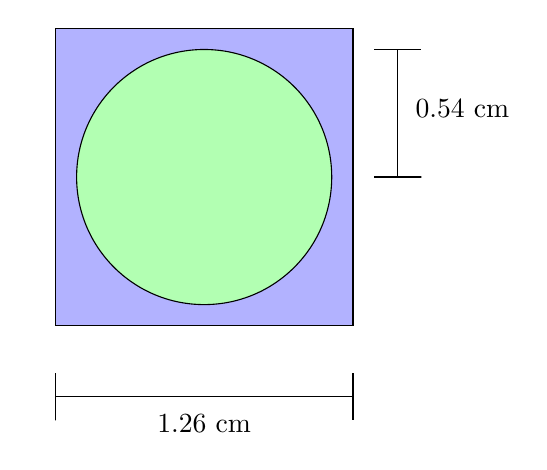
\begin{tikzpicture}[scale=3, every node/.style={scale=1}]
        \filldraw[xshift=0 cm, yshift=0 cm, fill=blue!30!white, draw=black] 
        (0, 0) rectangle (1.26,1.26) node[pos=.5] {};
        \filldraw[xshift=0 cm, yshift=0 cm, fill=green!30!white, draw=black] 
        (.63,.63) circle (.54) node[pos=.5] {};
        \draw (0,-.2) -- (0,-.4) -- (0,-.30) -- (0.63,-.3) node[below=0.1cm] 
        {1.26 cm} -- (1.26,-.30) -- (1.26,-.2) -- (1.26, -.4);
        \draw (1.35,.63) -- (1.55,.63) -- (1.45,.63) -- (1.45,.92) 
        node[right=0.1cm] {0.54 cm} -- (1.45,1.17) -- (1.35,1.17) -- (1.55, 
        1.17);
    \end{tikzpicture}
    \caption{Configuration for pincell.  The circular fuel element had a 
             radius of 0.54 cm and was homogenized with cladding for this 
             model.}
    \label{fig:pin_cell_config}
\end{figure*}
Here, the neutron transport equation for both 1-D and 2-D problems are solved by the discrete ordinates method, and all DMD calculations were performed using the PyDMD \cite{pydmd}.
An S4 Gauss-Legendre quadrature was used with the diamond difference approximation.
The reference eigenvalue and eigenvector were computed using full power iteration (i.e., fully converging the scattering source at each eigen iteration).

\section{Results for DMD-PM(n)}
As mentioned in the previous chapters, the major cost of the power method is from solving $\mathbf{Ax =b}$.
In this case, the computational time is proportional to the number of iterations.
Thus, the number of iterations is used as the indicator of computational cost in the following comparisons.

\subsection{Skipping Ahead with DMD-PM(n)}
As a first test of the method of DMD-PM($n$), the goal was to verify that DMD predicted eigenmodes prediction are closer to converged solutions.
A series of $n$ power iterations was performed to generate the snapshots, then the dominant eigenmode
was reconstructed as a function of iteration using \EQ{eq:dmd_predict}.
The absolute error with respect to the reference eigenmode was computed as the euclidean norm of the differences, or
\begin{equation}
 ||\mathbf{e}|| =  ||\mathbf{x}^{*}_i-\mathbf{x}_{ref}||_2   \, .
 \label{eq:error}
\end{equation}
The results shown in \FIGURE{fig:skipahead} are predicted using different number $n$ of snapshots where ``time'' is increasing.
Shown in parentheses is the number of equivalent power iterations to which the final, saturated error in the DMD prediction corresponds.
For example, application of 30 power iterations leads to a DMD surrogate that can predict an eigenmode with an accuracy equal to 149 power iterations, a substantial skip ahead in the number of iterations.

\begin{figure}[htb]%t=top, b=bottom, h=here
    \centering
    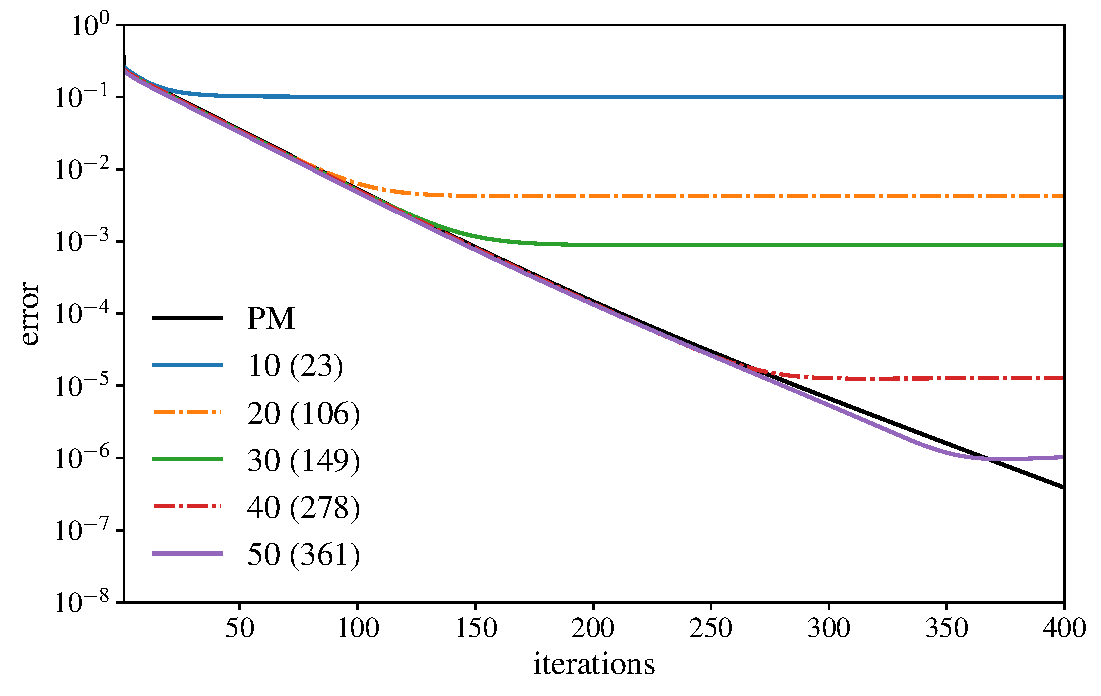
\includegraphics[height=4.0in]{tex/figures/skipahead.pdf}
   \caption{Error in the DMD-predicted, dominant eigenmode as a function of iteration.  The legend shows the number of power iterations $n$ used to construct the surrogate, and in parentheses is the effective number of power iterations the DMD surrogate can produce.}
  \label{fig:skipahead}
\end{figure}

The error shown in \FIGURE{fig:skipahead} approaches an asymptotic, lower bound as predictions are made beyond the number of power iterations used to generate the DMD surrogate.
As expected, a larger snapshots matrix can provide more information for learning the function and mapping a more accurate output.
Note that the final result reaching the lower bound here is very closed to the direct solution predicted by only the dominant DMD modes $\mathbf{\Phi_0}$, which demonstrate that our modified \EQUATION{eq:f_mode} can produce results with the same level of accuracy.

\subsection{Application of Restarted DMD-PM(n)}

As mentioned in \CHAPTER{chapter:DMD-PM}, the DMD-PM($n$) should restart from a set of snapshots multiple times until the solution converges.
To test the performance of the iterative application of the DMD-PM($n$) scheme, we used a fixed number $n$ at every restart to research the convergence.  
The results are shown in \FIGURE{fig:dmdpi_semilog}, which also includes the error for the unaccelerated PM and the Arnoldi method.
Here, the Arnoldi method was used without restarts. 
The results shown for the Arnoldi method are as a function of the size of the subspace used.

Note that the restart value for Restarted DMD-PM($n$) were selected as same as the skip ahead test.
Although a larger restart value can often yield a better acceleration, storing a larger number of snapshots uses more memory and requires more operations during the SVD decompostion.
Here, we consider the each DMD extrapolation process as an iteration on the horizontal, and, therefore, the final end points do not match exactly.

\begin{figure}[htb]%t=top, b=bottom, h=here
    \centering
    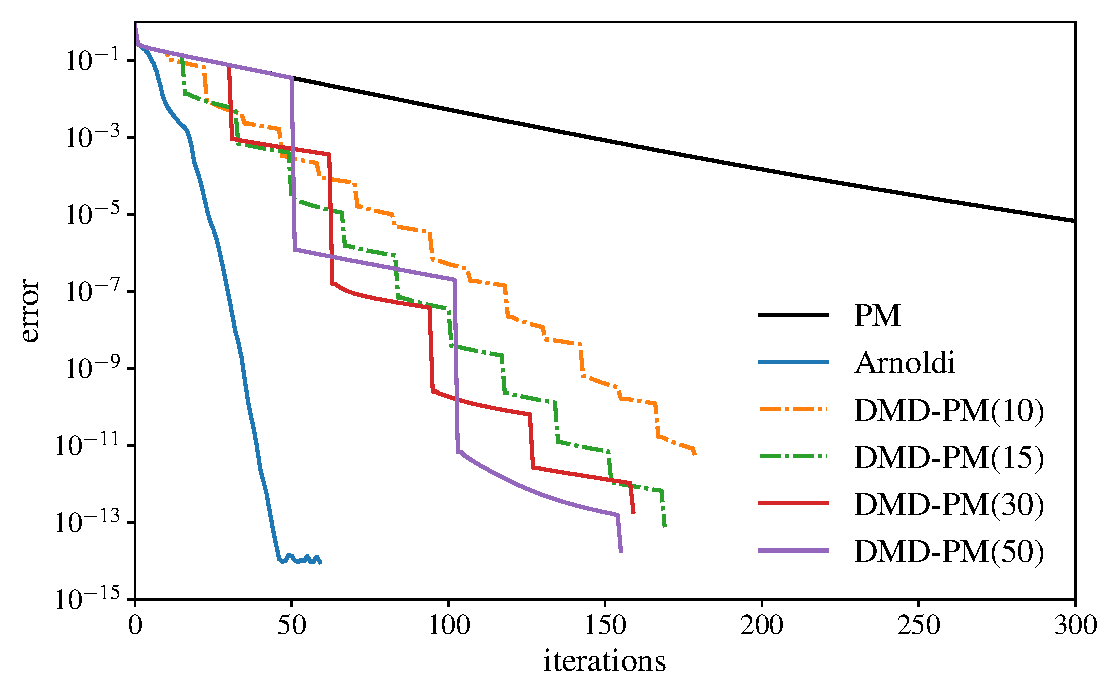
\includegraphics[height=4.0in]{tex/figures/dmdpi_semilog.pdf}
    \caption{The error in the predicted eigenmode for DMD-PM($n$), where $n$ is the number of power iterations performed.  Errors are also included for the power method (PM) and Arnoldi's method.}
    \label{fig:dmdpi_semilog}
\end{figure}

In this case, a tolerance of $10^{-14}$ is used as the tolerance for convergence.
For reference, approximately 800 unaccelerated power iterations are required to reach this error.
Ignoring the cost from DMD, the best DMD-PM($50$) only required around 150 iterations to reach the same error, thus providing (5$\times$) speedup compared to unaccelerated power iterations.

On the other hand, there is a significant performance difference between DMD-PM($n$) and the Arnoldi method, which is also expected.
The Arnoldi method only requires around 40 iterations to converge.
The Arnoldi method is based on a subspace that undergoes continuous orthonormalization, which produces a better-conditioned and, likely, richer basis than can be produced by successive application of $\mathbf{A}$ to a single vector.
Consequently, it is inapplicable when the explicit form of $\mathbf{A}$ is not available.  

\subsection{Restarted DMD-PM(n) for Higher Modes}
Note that DMD-PM($n$) is based on construction of Krylov subspace, therefore, it should be able to recover the higher-order modes approximately.
However, an unrestarted DMD-PM approximation produces to an ill-conditioned basis and, hence, cannot produce approximations for higher-order modes with reliable accuracy.
Moreover, the iterative DMD-PM($n$) using \EQ{eq:f_mode} throws away all higher-order modes upon the restart.
In order to reconstruct the higher-order modes, the dominant mode was kept with a small contribution from the next two modes in order to capture the three modes with the largest eigenvalues, instead of using only the dominant DMD modes.
Specifically, the initial guess at each restarts was computed by $\mathbf{x}_0 + \epsilon ( \mathbf{x}_1 + \mathbf{x}_2)$, where $\epsilon$ is a small value (here, $10^{-4}$).
Consequently, the next iteration contains some contribution from the higher-order space.

The reference modes are shown in Figure~\ref{fig:ref_modes}.
The largest three eigenvalues and their corresponding modes were recovered using the second, third, or fourth iterations of DMD-PM($30$) as approximations for the first three eigenpairs of the original system.
Errors in higher-order mode estimates were found to depend on the randomized initial guess for the first power iteration, and the representative values of the absolute errors in the DMD-PM($n$) approximations are shown in Figure~\ref{fig:appx_modes}, where computed eigenvectors were normalized to unity. 

As can be observed, the error in the dominant mode after two iterations ($1.77\times 10^{-7}$) is nearly unchanged from the case in which higher modes are not kept ($1.54\times 10^{-7})$; see Figure \ref{fig:dmdpi_semilog}.
However, the performance does degrade somewhat thereafter, with errors after three and four iterations of approximately $4.94\times 10^{-9}$ and $1.38\times 10^{-10}$, respectively, compared to $9.90\times 10^{-11}$ and $3.00\times 10^{-12}$ in Figure~\ref{fig:dmdpi_semilog}.

The absolute errors in the two higher-order modes (and their eigenvalues) are much larger than the error for the dominant mode, similarly, these errors are also decreasing with each iteration.
The third and fourth iteration also degrade for the two higher-order modes, especially the third largest eigenpairs. 
The error of the second order modes reach $1.28\times 10^{-3}$, and still provide fair improvement in the fourth iteration.
Meanwhile, the error of the third order eigenpair only reach $5.18\times 10^{-2}$ after 3 iterations and keep in a same level in the next iteration.

\begin{figure*}[htb]
 \centering
    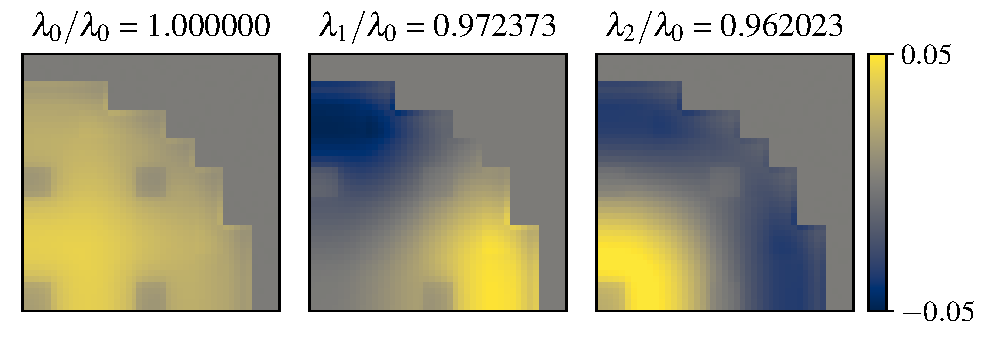
\includegraphics[width=0.64\textwidth]{tex/figures/ref_modes.pdf}\\
    \caption{First three reference eigenmodes; the corresponding eigenvalue ratios are shown above.}
    \label{fig:ref_modes}
\end{figure*}

\begin{figure*}[!]
 \begin{subfigure}[b]{\textwidth}
  \centering
    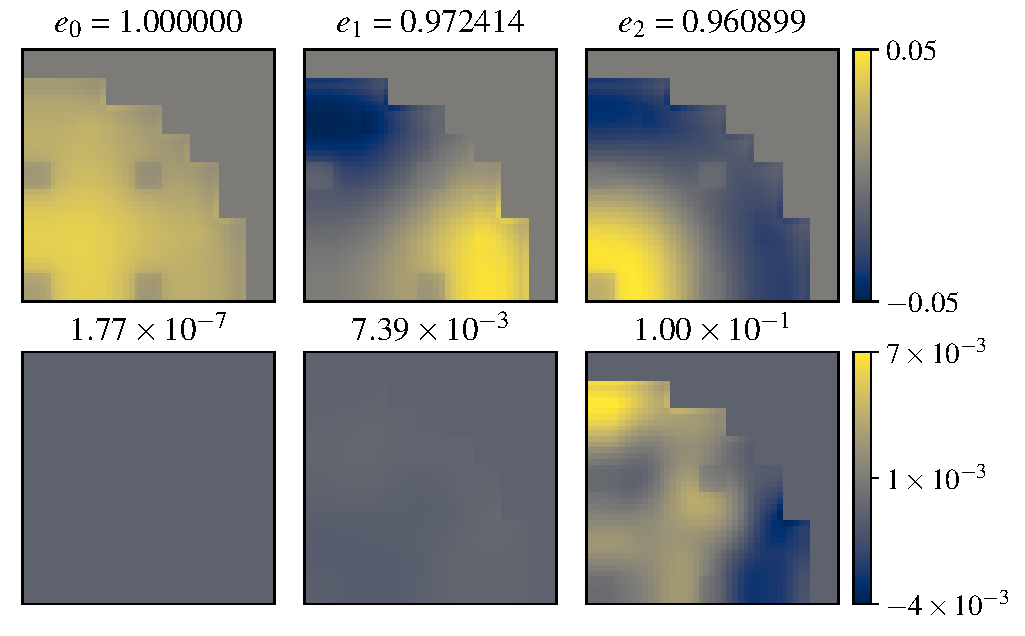
\includegraphics[width=0.60\textwidth]{tex/figures/appx_modes_2_3.pdf}\\
    \caption{Two iterations of DMD-PI(30) with retention of 3 approximate modes.}
    \label{fig:appx_modes_2_3}
 \end{subfigure}
 
 \begin{subfigure}[b]{\textwidth}
  \centering
   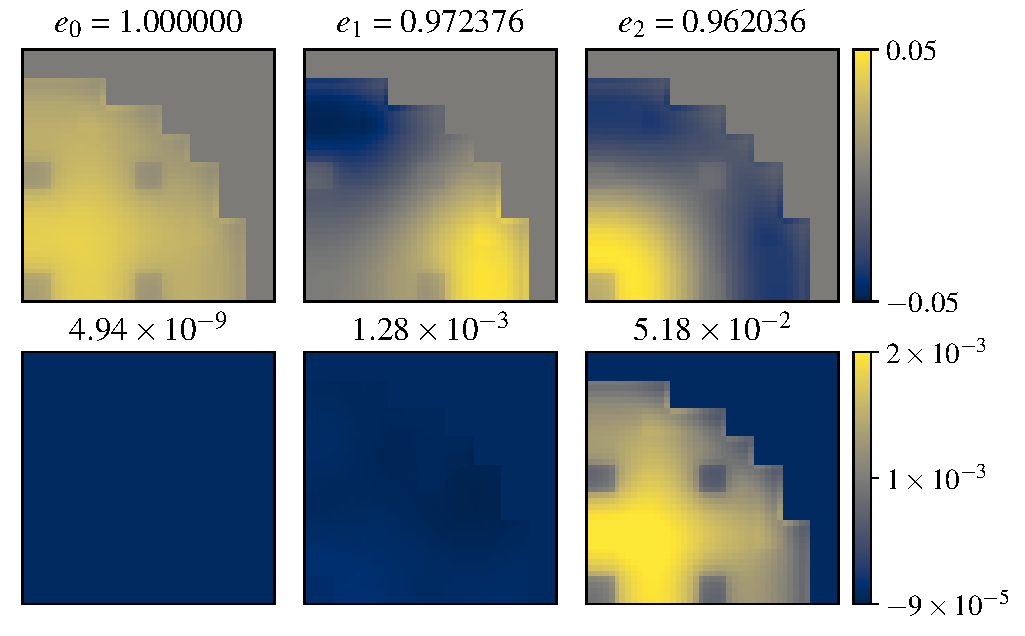
\includegraphics[width=0.60\textwidth]{tex/figures/appx_modes_3_3.pdf}\\
   \caption{Three iterations of DMD-PI(30) with retention of 3 approximate modes.}
   \label{fig:appx_modes_3_3}
 \end{subfigure}
 
 \begin{subfigure}[b]{\textwidth}
  \centering
   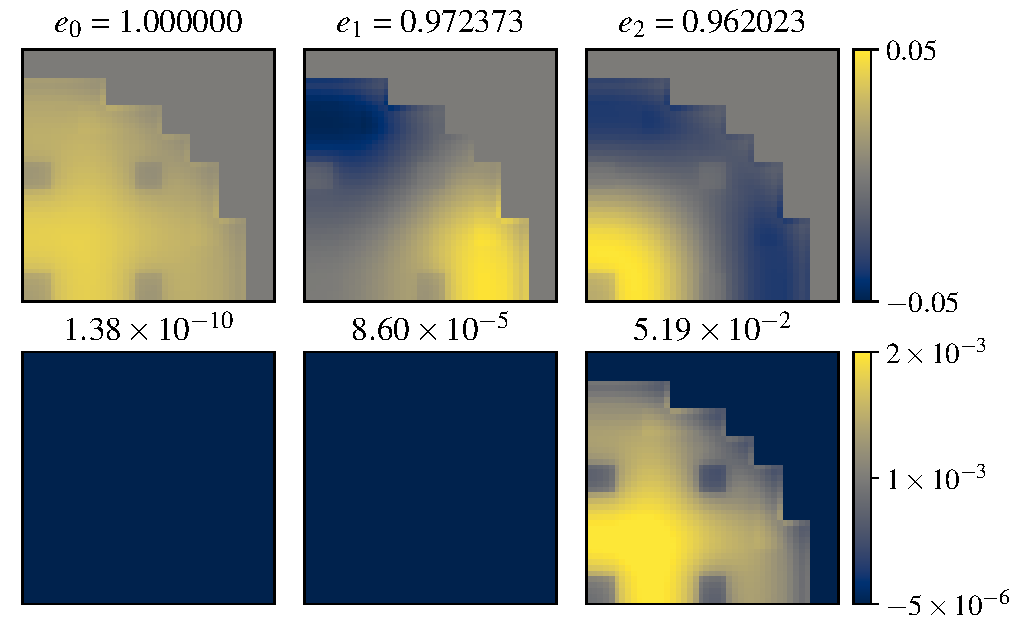
\includegraphics[width=0.60\textwidth]{tex/figures/appx_modes_4_3.pdf}\\
   \caption{Four iterations of DMD-PI(30) with retention of 3 approximate modes.}
   \label{fig:appx_modes_4_3}
 \end{subfigure}
 \caption{Shown in the top row of each subfigure are the first three modes as computed from several applications of DMD-PM($30$).   The second row shows the error $\mathbf{e}_i = \mathbf{x}_i^{\text{reference}}-\mathbf{x}_i^{\text{approximate}}$.  The corresponding $e_i \approx \lambda_i/\lambda_0$ (top row) and norm of the error $||\mathbf{e}_i||_2$ (bottom row) are also shown.}
 \label{fig:appx_modes}
\end{figure*}

\section{Results for DMD-FPM(n)}

As mentioned in the \CHAPTER{chapter:PM}, the flattened PM eliminates the inner iterations and only apply one transport sweep each iteration.
Therefore, we used number of sweeps as the measure for the total computational cost, which is equivalent to number of iterations.
Two similar tests on different geometries are conducted and solved for a variety of restart values $n$ to study the optimum condition.
The reference solutions were computed using full power method (i.e.,fully converging the scattering source at each eigen iteration).
The error is defined as same as \EQUATION{eq:error}, and the tolerance of convergence is set as $10^{-8}$.

\subsection{DMD-FPM(n) for 1D BWR Test Problem}

To compare performance, the generalized $k-$eigenvalue problem was solved first by flattened power iteration, which used 3445 transport sweeps for this BWR problem.
The best DMD-FPM($n$) algorithm used 40 snapshots, and required approximately 270 transport sweeps, thus providing more than an order of magnitude reduction in the computational cost.

\begin{figure}[htb]%t=top, b=bottom, h=here
    \centering
    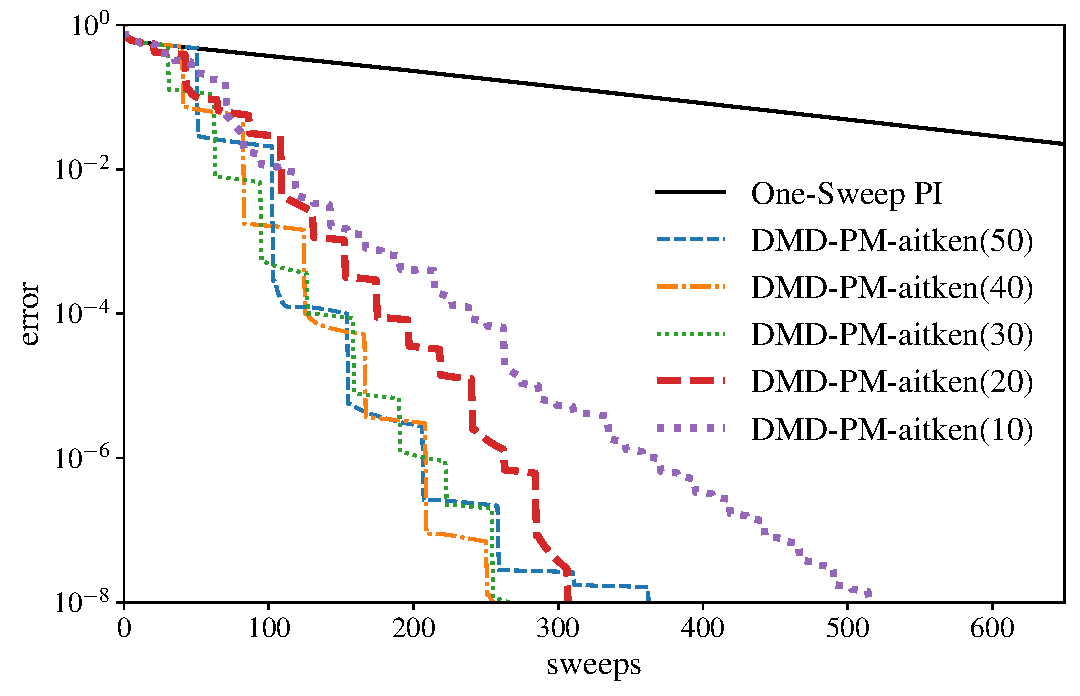
\includegraphics[height=4.0in]{tex/figures/dmd_ospi_semilog_1d.pdf}
    \caption{The absolute error in the predicted eigenmode for DMD-PM-aitken(n) for the 1D BWR problem, where n is the number of transport sweeps performed.}
    \label{fig:DMD-FPM_1d}
\end{figure}

This case shows that using a larger number of snapshots cannot promise a faster convergence for DMD-FPM($n$).
The reason might be the error remaining from dismatched eigenvalues.

\subsection{DMD-FPM(n) for 2D C5G7 Test Problem}

Similar the 1-D results, the results of C5G7 2-D benchmark also show that the best condition of DMD-FPM($n$) algorithm has significant speedup compared to flattened power iteration, which required 351 transport sweep to reduce error to $1e-8$ while using 30 snapshots each restart.
For reference, approximately 1570 unaccelerated flattened power sweeps are required for this problem to be fully converged.
As expected in this case, a small increase in error may be observed more obviously for each application of DMD-FPM($n$) due to the previously discussed eigenvalue error.
And the best case is not using the most number of snapshots, though the difference of sweeps is relatively small.

\begin{figure}[htb]%t=top, b=bottom, h=here
    \centering
    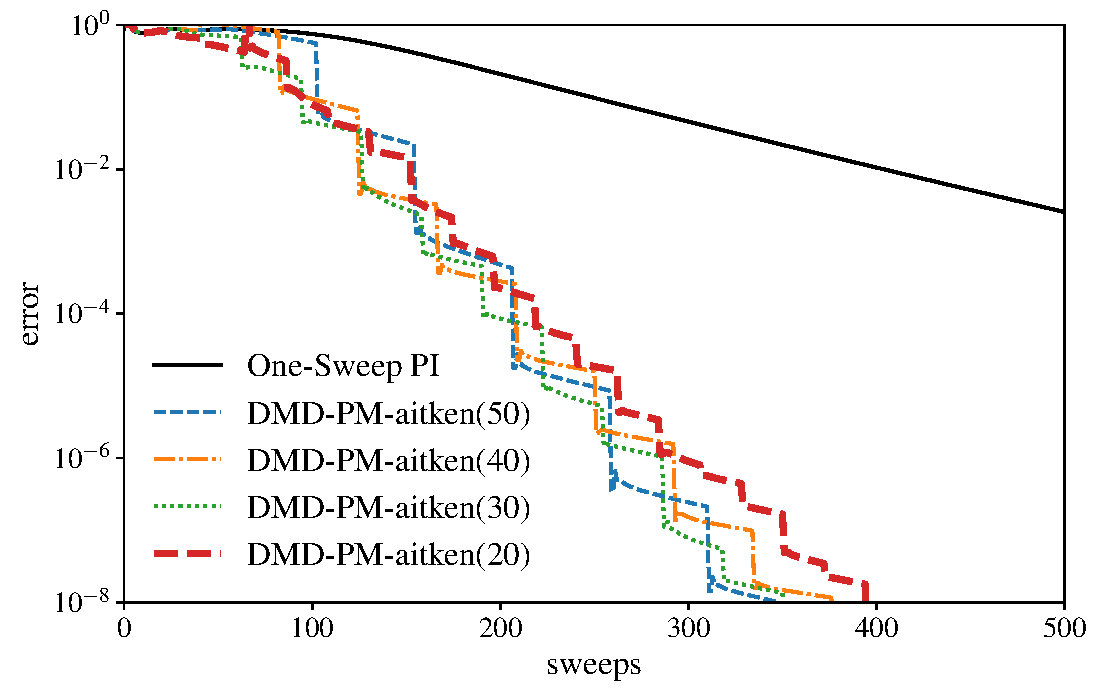
\includegraphics[height=4.0in]{tex/figures/dmd_ospi_semilog_c5g7.pdf}
    \caption{The absolute error in the predicted eigenmode for DMD-PM-Aitken(n) for the 2D C5G7 problem, where n is the number of transport sweeps performed.}
    \label{fig:DMD-FPM_2d}
\end{figure}

Using DMD too frequently (i.e., small $n$) might produce a large numerical error from SVD decomposition, the error increase many level of magnitude from DMD.
This is the reason why DMD-FPM($10$) did not reduce the error to within the target range.
The number of transport sweeps required to reach a tolerance of $10^{-8}$ are shown in \TAB{tab:widetable}.

\begin{table*}[htb]
  \centering
  \small
  \caption{Number of transport sweep}
  \begin{tabular}{lllllllll}\toprule
      & FPM  & DMD-FPM(10)& DMD-FPM(20)& DMD-FPM(30)& DMD-FPM(40)& DMD-FPM(50)
\\ \midrule
$BWR$  & 3444 & 515 & 307 & 267 & 256 & 363
\\
$C5G7$  & 1570  & N/A & 395 & 351 & 377 & 395
\\
\bottomrule
\end{tabular}
  \label{tab:widetable}
\end{table*}
